%!TEX program = xelatex
\documentclass[a4paper,UTF8]{ctexart}
\usepackage[unicode=true,colorlinks,urlcolor=blue,linkcolor=blue,bookmarksnumbered=true]{hyperref}
\usepackage{latexsym,amssymb,amsmath,amsbsy,amsopn,amstext,amsthm,amsxtra,color,multicol,bm,calc,ifpdf}
\usepackage{graphicx}
\usepackage{diagbox}   % 绘制表格斜线
\usepackage{enumerate}
\usepackage{epstopdf}
\usepackage{fancyhdr}
\usepackage{subfigure}
\usepackage{listings}
\usepackage{multirow}
\usepackage{makeidx}
\usepackage{xcolor} 
\usepackage{fontspec}                            % 建立索引宏包
\graphicspath{{figures/}}  % 设置图片搜索路径
\theoremstyle{plain} \newtheorem{theorem}{定理}[section]
\theoremstyle{plain} \newtheorem{definition}{定义}[section]
\theoremstyle{plain} \newtheorem{lemma}{引理}[section]
\theoremstyle{plain} \newtheorem{proposition}{命题}[section]
\theoremstyle{plain} \newtheorem{example}{例}[section]
\theoremstyle{plain} \newtheorem{remark}{注}[section]
\theoremstyle{plain} \newtheorem{corollary}{推论}[section]
\newfontfamily\courier{Courier New}
\lstset{linewidth=1.1\textwidth,
        numbers=left, %设置行号位置 
        basicstyle=\small\courier,
        numberstyle=\tiny\courier, %设置行号大小  
        keywordstyle=\color{blue}\courier, %设置关键字颜色  
        %identifierstyle=\bf,
        commentstyle=\it\color[cmyk]{1,0,1,0}\courier, %设置注释颜色 
        stringstyle=\it\color[RGB]{128,0,0}\courier,
        %framexleftmargin=10mm,
        frame=single, %设置边框格式  
        backgroundcolor=\color[RGB]{245,245,244},
        %escapeinside=``, %逃逸字符(1左面的键),用于显示中文  
        breaklines, %自动折行  
        extendedchars=false, %解决代码跨页时,章节标题,页眉等汉字不显示的问题  
        xleftmargin=2em,xrightmargin=2em, aboveskip=1em, %设置边距  
        tabsize=4, %设置tab空格数  
        showspaces=false %不显示空格  
        basicstyle=\small\courier
       }  
\newenvironment{mysolution}{{\color{blue} 解}: }{{\color{magenta}\qed}}
\newcommand\diff{\,{\mathrm d}} %定义微分d
\newcommand{\p}[3]{\frac{\partial^{#1}#2}{\partial{#3}^{#1}}}  %定义求偏导算子
\newcommand{\ucite}[1]{\textsuperscript{\cite{#1}}}  %参考文献引用:上标用\ucite{ },文中用\cite{ }

\begin{document}
\title{

\includegraphics[width=0.65\textwidth]{onepiece.pdf}\\
\vspace{2em}
\textbf{关联规则学习笔记}}
\author{\emph{李向阳} \quad {\color{blue} d1142845997@gmail.com}
}
\date{}


\maketitle
\thispagestyle{empty}

\newpage


\tableofcontents

\newpage

\section{引入}
这一次讲讲关联规则(Association Rules, AR).

关联式规则, 又称关联规则, 是数据挖掘的一个重要课题, 用于从大量数据中挖掘出有价值的数据项之间的相关关系. 关联规则解决的常见问题如: “如果一个消费者购买了产品A, 那么他有多大机会购买产品B?”以及“如果他购买了产品C和D, 那么他还将购买什么产品?”正如大多数数据挖掘技术一样, 关联规则的任务在于减少潜在的大量杂乱无章的数据, 使之成为少量的易于观察理解的静态资料. 关联式规则一般考虑项目的次序, 而仅考虑其组合.

关联规则一个经典的实例是购物篮分析(Market Basket Analysis). 超市对顾客的购买记录数据库进行关联规则挖掘, 可以发现顾客的购买习惯, 例如, 购买产品X的同时也购买产品Y(比如网球与网球拍等等), 于是超市就可以调整货架的布局, 比如将X产品和Y产品放在一起来增进销量. 当然, 最广为人知的还是啤酒与尿布的例子, 即超市发现很多购买者经常同时购买这两种商品, 后来得知, 美国的妇女们经常会嘱咐她们的丈夫下班后为孩子买尿布, 而丈夫在买完尿布后又要顺手买回自己爱喝的啤酒, 因此啤酒和尿布在一起被购买的机会很多.

诸如此类的案例很多, 而且我们看到, 关联规则有一点推荐算法的味道, 所以它在电商、互联网等领域确实很有用, 是数据挖掘的一个经典算法.下面就来稍微系统的介绍一些概念和常用的算法.


\section{基本概念}
在关联规则中, 我们把物品(Item)称为项, 同推荐算法一样, 我们设有$n$个物品, 即项的集合为$I = \{i_1,i_2,\cdots,i_n\}$. 那么这里的样本是什么呢?

当然还是人的行为了, 这里一般是购买行为, 还是设有$m$个样本, 记为$\bm{t}_{i}$, 它是项集$I$的非空子集, 表示第$i$个人购买了哪些物品. 用数据挖掘的术语来说, 我们称集合$D = \{\bm{t}_1,\bm{t}_2,\cdots,\bm{t}_m\}$为一个交易数据库, 而每一个$\bm{t}_i$称为一个事务(Transaction)或者交易(其实就是一个用户的购买记录).每一个事务都用一个唯一的标识符, 即事务的ID(Transaction ID)表示, 简记为 TID. 

所谓关联规则, 是指形如$X \Rightarrow Y$的蕴涵式, 其中$X,Y \subseteq I$且$X \cap Y = \emptyset$, $X$和$Y$分别称为关联规则的先导(antecedent或left-hand-side, LHS)和后继(consequent或right-hand-side, RHS).

显然, 并不是任何一个关联规则都是我们感兴趣的, 需要对关联规则加一些约束, 为此我们引入支持度(Support)和置信度(Confidence)的定义.

关联规则$X \Rightarrow Y$的支持度是指$D$中事务包含$X \cup Y$的百分比, 即$X$和$Y$同时出现的概率$P(X \cup Y)$.
\begin{equation*}
\mathrm{Support}(X \Rightarrow Y) = P(X \cup Y) = \frac{|X \cup Y|}{|D|} = \frac{|X \cup Y|}{m}
\end{equation*}

注意这里的$X \cup Y$表示$X, Y$同时出现. 此外, 我们一般把$|X \cup Y|$称作项集$\{X,Y\}$的绝对支持度, 除以$m$后称为相对支持度.

关联规则$X \Rightarrow Y$的置信度是指包含$X$的事务中同时包含$Y$的百分比, 即条件概率$P(Y | X)$.
\begin{equation*}
\mathrm{Confidence}(X \Rightarrow Y) = P(Y | X) = \frac{|X \cup Y|}{|X|}
\end{equation*}

一般情况下我们会给支持度和置信度定一个下限(阈值), 称为最小支持度和最小置信度. 如果一个关联规则同时满足最小支持度和最小置信度, 则认为这个关联规则是有趣的, 并称其为强关联规则(Strong Association Rules).

说了这么多抽象的概念, 来举个例子. 下表\ref{tennis}是顾客购买记录的数据库$D$, 包含$6$个事务(也就是包含$m = 6$个样本). 其中包含$n = 4$个物品, 即项集$I = \{\textrm{网球拍, 网球, 运动鞋, 羽毛球}\}$. 我们给定最小支持度$\alpha = 0.4$, 最小置信度$\beta = 0.6$(这个暂时是随便定的).
\begin{table}[!htb]
\centering
\caption{网球拍与网球}
\label{tennis}
\begin{tabular}{c|c|c|c|c}
	\hline
    % after \: \hline or \cline{col1-col2} \cline{col3-col4} ...
    \textbf{TID} & \textbf{网球拍} & \textbf{网球} & \textbf{运动鞋} & \textbf{羽毛球} \\
    \hline
    T1 & 1 & 1 & 1 & 0 \\
    \hline
    T2 & 1 & 1 & 0 & 0 \\
    \hline
    T3 & 1 & 0 & 0 & 0 \\
    \hline
    T4 & 1 & 0 & 1 & 0 \\
    \hline
    T5 & 0 & 0 & 1 & 1 \\
    \hline
    T6 & 1 & 1 & 0 & 0 \\
	\hline
\end{tabular}
\end{table}

这里我们用$1$表示购买了商品, 用$0$表示没有购买该商品.

考虑关联规则: 网球拍 $\Rightarrow$ 网球, 这是不是一个强关联规则呢?

我们来计算一下. 事务T1,T2,T3,T4,T6 包含网球拍, 事务T1,T2,T6 同时包含网球拍和网球, 所以支持度$\mathrm{Support}(\textrm{网球拍} \Rightarrow \textrm{网球}) = 3 / 6 = 0.5 \geqslant \alpha$, 置信度$\mathrm{Confidence}(\textrm{网球拍} \Rightarrow \textrm{网球}) = 3 / 5 = 0.6 \geqslant \beta$, 所以它是强关联规则, 也就是可认为购买网球拍和购买网球之间存在强关联.

以上我们是把所有样本用矩阵表示了出来, 很类似于推荐算法中的评分矩阵, 但是生活中的很多数据并不是这样给出的, 可能更类似于 Python 中字典的存储方式. 比如如下表\ref{beers}, 也就是啤酒与尿布的例子.
\begin{table}[!htb]
\centering
\caption{啤酒与尿布}
\label{beers}
\begin{tabular}{c|l}
	\hline
    % after \: \hline or \cline{col1-col2} \cline{col3-col4} ...
    \textbf{TID} & \textbf{Items}  \\
    \hline
    T1 & \{牛奶, 面包\}  \\
    \hline
    T2 & \{面包, 尿布, 啤酒, 鸡蛋\}  \\
    \hline
    T3 & \{牛奶, 尿布, 啤酒, 可乐\}  \\
    \hline
    T4 & \{面包, 牛奶, 尿布, 啤酒\}  \\ 
    \hline
    T5 & \{面包, 牛奶, 尿布, 可乐\}  \\
	\hline
\end{tabular}
\end{table}

关联规则挖掘的任务便是找出所有的强关联规则, 以便于公司或者超市更好的决策. 那么如何找到所有的强关联规则呢? 这就有很多算法. 下面就来稍微介绍一些常用的算法.


\section{关联规则算法}
仔细想一下, 对于关联规则$X \Rightarrow Y$, 不管是计算支持度还是置信度, 最关键的还是计算$\{X,Y\}$同时出现的次数, 即它们交集的绝对支持度, 所以我们一般把关联规则挖掘分两步进行:
\begin{enumerate}[(1)]
\item 找出所有满足绝对最小支持度的项目集, 称为频繁项集(Frequent Item Sets)

\item 在频繁项集的基础上生成满足最小置信度的规则, 从而产生强关联规则
\end{enumerate}

我们一般把项(物品)的集合称为项集, 包含$k$个项的集称为$k$项集. 满足绝对最小支持度的项集(即项目集出现的次数不小于绝对最小支持度), 称为频繁项集. 比如对表\ref{beers}来说, 给定绝对最小支持度$\alpha = 3$, 那么容易看出所有的频繁项集有$6$个, 其中频繁$1$项集是{牛奶:4}和{面包:4}, 频繁$2$项集是{面包, 尿布:3}, {尿布, 牛奶:3}, {面包, 牛奶:3} 和 {尿布, 啤酒:3}.

关联规则挖掘所花费的时间主要是在第一步, 也就是生成频繁项集上, 因为找出的频繁项集往往不会很多, 因此第二步利用频繁项集生成规则也就不会花太多的时间,而生成频繁项集需要测试很多的备选项集, 所以大量的算法主要是解决第一步的. 下面介绍的算法主要就是如何生成频繁项集.


\subsection{Apriori 算法}
为了减少频繁项集的生成时间, 我们应该尽早的消除一些完全不可能是频繁项集的集合, Apriori的两条定理就是干这事的.

Apriori定理1: 如果一个集合是频繁项集, 则它的所有子集都是频繁项集. 举例: 假设一个集合\{A,B\}是频繁项集, 即A、B同时出现在一条记录的次数大于等于绝对最小支持度, 则它的子集\{A\},\{B\}出现次数也必定大于等于绝对最小支持度, 即它的子集都是频繁项集.

Apriori定理2: 如果一个集合不是频繁项集, 则它的所有超集都不是频繁项集. 举例: 假设集合\{A\}不是频繁项集, 即A出现的次数小于绝对最小支持度, 则它的任何超集如\{A,B\}出现的次数必定也小于绝对最小支持度, 因此其超集必定也不是频繁项集.

利用这两条定理, 我们抛掉很多的候选项集, Apriori算法就是利用这两个定理来实现快速挖掘频繁项集的.

Apriori是由A priori合并而来的, 它的意思是后面的是在前面的基础上推出来的, 即先验推导, 其实就是二级频繁项集是在一级频繁项集的基础上产生的, 三级频繁项集是在二级频繁项集的基础上产生的, 以此类推.

Apriori算法属于候选消除算法, 是一个生成候选集、消除不满足条件的候选集、并不断循环直到不再产生候选集的过程. 还是以表\ref{beers}为例, 设定绝对最小支持度$\alpha = 3$, 下面用图来说明 Apriori算法的过程, 见图\ref{apbeers}.
\begin{figure}[!htb]
	\centering
	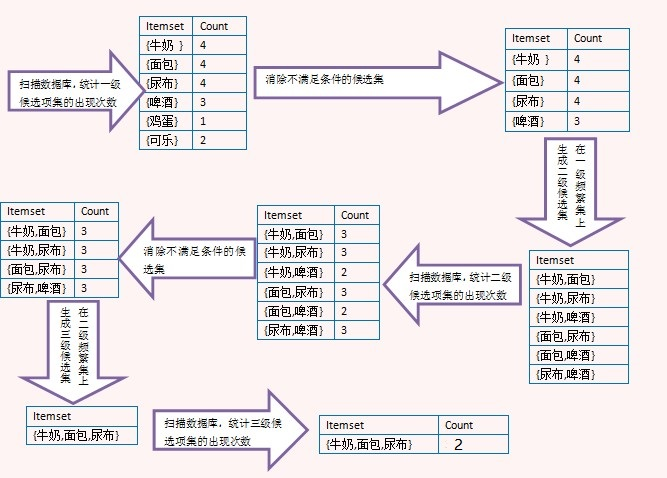
\includegraphics[width = 0.85 \textwidth]{beers.jpg}
	\caption{Apriori 算法过程示例}
	\label{apbeers}
\end{figure}

上面的图演示了Apriori算法的过程, {\color{red}注意看由二级频繁项集生成三级候选项集时, 没有\{牛奶,面包,啤酒\}, 那是因为\{面包,啤酒\}不是二级频繁项集, 这里利用了Apriori定理}. 最后生成三级候选项集后, 发现\{牛奶, 面包, 尿布\}不是频繁项集, 因此也就没有更高一级的候选项集了, 整个算法结束.

维基上也有一个示例, 几乎是完全类似的, 可见\url{https://zh.wikipedia.org/zh/%E5%85%B3%E8%81%94%E5%BC%8F%E8%A7%84%E5%88%99}. 我们也来说明一下. 假设有一个数据库$D$, 其中有$4$个事务, 可见下表
\begin{table}[!htb]
\centering
\caption{维基数据集}
\label{wiki}
\begin{tabular}{c|l}
	\hline
    % after \: \hline or \cline{col1-col2} \cline{col3-col4} ...
    \textbf{TID} & \textbf{Items}  \\
    \hline
    T1 & I1, I3, I4 \\
    \hline
    T2 & I2, I3, I5 \\
    \hline
    T3 & I1, I2, I3, I5 \\
    \hline
    T4 & I2, I5 \\
	\hline
\end{tabular}
\end{table}

其中I1到I5表示商品, 这里预定绝对最小支持度 minSupport = 2, 下面运用 Apriori 算法来找出所有的频繁项集.

首先扫描$D$, 对每个候选项进行绝对支持度计数得到下表\ref{c1}.
\begin{table}[!htb]
\centering
\caption{表 	C1}
\label{c1}
\begin{tabular}{c|c}
	\hline
    % after \: \hline or \cline{col1-col2} \cline{col3-col4} ...
    \textbf{项集} & \textbf{支持度计数}  \\
    \hline
    \{I1\}   &  2  \\
    \hline
    \{I2\}   &  3  \\
    \hline
    \{I3\}   &  3 \\
    \hline
    \{I4\}   &  1  \\
    \hline
    \{I5\}   &  3  \\
	\hline
\end{tabular}
\end{table}

比较候选项与最小支持度 minSupport, 产生$1$维频繁项集 L1:
\begin{table}[!htb]
\centering
\caption{表 L1}
\label{l1}
\begin{tabular}{c|c}
	\hline
    % after \: \hline or \cline{col1-col2} \cline{col3-col4} ...
    \textbf{项集} & \textbf{支持度计数}  \\
    \hline
    \{I1\}   &  2 \\
    \hline
    \{I2\}   &  3 \\
    \hline
    \{I3\}   &  3 \\
    \hline
    \{I5\}   &  3 \\
	\hline
\end{tabular}
\end{table}

由 L1 产生候选项集 C2, 并扫描数据库$D$, 对每个候选项集进行支持度计数, 得表\ref{c2}.
\begin{table}[!htb]
\centering
\caption{表 C2}
\label{c2}
\begin{tabular}{c|c}
	\hline
    % after \: \hline or \cline{col1-col2} \cline{col3-col4} ...
    \textbf{项集} & \textbf{支持度计数}  \\
    \hline
    \{I1, I2\}   &   1  \\
    \hline
    \{I1, I3\}   &   2  \\
    \hline
    \{I1, I5\}   &   1  \\
    \hline
    \{I2, I3\}   &   2  \\
    \hline
    \{I2, I5\}   &   3  \\
    \hline
    \{I3, I5\}   &   2  \\
	\hline
\end{tabular}
\end{table}

比较候选项支持度计数与最小支持度 minSupport, 产生$2$维频繁项集 L2, 可见表\ref{l2}.
\begin{table}[!htb]
\centering
\caption{表 L2}
\label{l2}
\begin{tabular}{c|c}
	\hline
    % after \: \hline or \cline{col1-col2} \cline{col3-col4} ...
    \textbf{项集} & \textbf{支持度计数}  \\
    \hline
    \{I1, I3\}   &   2  \\
    \hline
    \{I2, I3\}   &   2  \\
    \hline
    \{I2, I5\}   &   3  \\
    \hline
    \{I3, I5\}   &   2  \\
	\hline
\end{tabular}
\end{table}

由 L2 产生候选集 C3 ({\color{red}注意此步也只产生一个候选项, 道理同上面的那个例子是一样的}), 并扫描数据库$D$, 对每个候选项集进行支持度计数
\begin{table}[!htb]
\centering
\caption{表 C3}
\label{c3}
\begin{tabular}{c|c}
	\hline
    % after \: \hline or \cline{col1-col2} \cline{col3-col4} ...
    \textbf{项集} & \textbf{支持度计数}  \\
    \hline
    \{I2, I3, I5\}   &  2  \\
	\hline
\end{tabular}
\end{table}

比较候选项支持度计数与最小支持度 minSupport, 可知上面的\{I2, I3, I5\}是一个$3$频繁项集, 算法终止.


\subsection{FP-Growth 算法}
Aprori算法是一个经典算法, 其利用频繁集的两个特性, 过滤了很多无关的集合, 其优点是简单、易理解、数据要求低, 但是我们发现Apriori算法是一个候选消除算法, 每一次消除都需要扫描一次所有数据记录, 造成整个算法在面临大数据集时显得无能为力. 下面就来介绍 FP-Growth(Frequent Pattern Growth) 算法, 它的效率比 Aprori 算法高很多. 

FP-Growth算法通过构造一个树结构来压缩数据记录, 是一种不产生候选项集而采用频繁项集增长的方法挖掘频繁项集的算法. 算法只需要扫描2次数据库: 第一次扫描数据库, 得到$1$维频繁项集; 第二次扫描数据库, 利用$1$维频繁项集过滤数据库中的非频繁项, 同时生成FP树(Frequent Pattern Tree). 由于FP树蕴涵了所有的频繁项集, 其后的频繁项集的挖掘只需要在FP树上进行. FP树挖掘由两个阶段组成: 第一阶段建立FP树, 即将数据库中的事务构造成一棵FP树; 第二阶段为挖掘FP树, 即针对FP树挖掘频繁项集和关联规则.

为了说明整个过程, 我们还是以表\ref{beers}中的数据举例, 设定绝对最小支持度 minSupport = 3.

\subsubsection{构造 FP-Tree}
树的每一个结点代表一个项, 这里我们先不着急看树的结构,先来演示一下FP-Tree的构造过程, FP-Tree构造好后自然明白了树的结构.

\noindent \textbf{Step 1}: 扫描数据记录, 生成一级频繁项集, 并按出现次数由多到少排序, 如下表\ref{step1}所示.
\begin{table}[!htb]
\centering
\caption{一级频繁项集}
\label{step1}
\begin{tabular}{c|c}
	\hline
    % after \: \hline or \cline{col1-col2} \cline{col3-col4} ...
    \textbf{Item} & \textbf{Count}  \\
    \hline
    牛奶   &  4  \\
    \hline
    面包   &  4  \\
    \hline
    尿布   &  4  \\
    \hline
    啤酒   &  4  \\
	\hline
\end{tabular}
\end{table}

可以看到, 鸡蛋和可乐没有出现在上表中, 因为可乐只出现2次, 鸡蛋只出现1次, 均小于最小支持度, 因此不是频繁项集, 根据Apriori定理, 非频繁项集的超集一定不是频繁项集, 所以可乐和鸡蛋不需要再考虑.


\noindent \textbf{Step 2}: 再次扫描数据记录, 对每条记录中出现在\textbf{Step 1}产生的表中的项, 按表中的顺序排序. 初始时, 新建一个根结点, 标记为null, 设置 count 为$-1$(只是为了与其他区分开来).

\begin{enumerate}[(1)]
\item 第一条记录: \{牛奶,面包\}

按\textbf{Step 1}表过滤排序得到依然为\{牛奶,面包\}, 新建一个结点, idName为{牛奶}, 将其插入到根节点下, 并设置count为1, 然后新建一个\{面包\}结点, 插入到{牛奶}结点下面, 插入后如下图\ref{tree1}所示:
\begin{figure}[!htb]
	\centering
	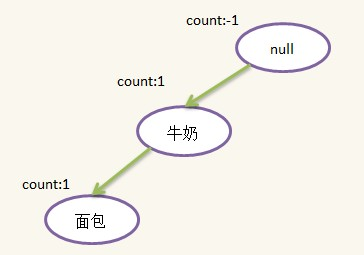
\includegraphics[width = 0.75 \textwidth]{tree1.jpg}
	\caption{第一条记录}
	\label{tree1}
\end{figure}


\item 第二条记录: \{面包,尿布,啤酒,鸡蛋\}

过滤并排序后为: \{面包,尿布,啤酒\}, 发现根结点没有包含\{面包\}的儿子(虽然有一个\{面包\}的孙子但不是儿子), 因此新建一个\{面包\}结点, 插在根结点下面, 这样根结点就有了两个孩子, 随后新建\{尿布\}结点插在\{面包\}结点下面, 新建\{啤酒\}结点插在\{尿布\}下面, 插入后如下图\ref{tree2}所示.
\begin{figure}[!htb]
	\centering
	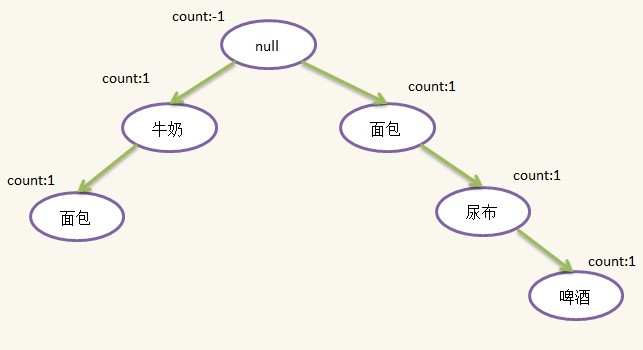
\includegraphics[width = 0.75 \textwidth]{tree2.jpg}
	\caption{第二条记录}
	\label{tree2}
\end{figure}

\item 第三条记录: \{牛奶,尿布,啤酒,可乐\}

过滤并排序后为: \{牛奶,尿布,啤酒\}, 这时候发现根结点有儿子\{牛奶\}, 因此不需要新建结点, 只需将原来的\{牛奶\}结点的count加1即可, 往下发现\{牛奶\}结点有一个儿子\{尿布\}, 于是新建\{尿布\}结点, 并插入到\{牛奶\}结点下面, 随后新建\{啤酒\}结点插入到\{尿布\}结点后面, 插入后如下图\ref{tree3}所示.
\begin{figure}[!htb]
	\centering
	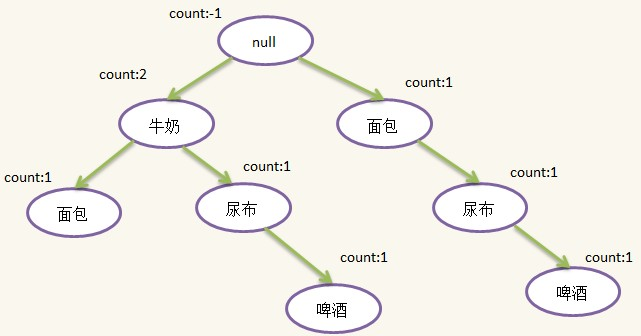
\includegraphics[width = 0.75 \textwidth]{tree3.jpg}
	\caption{第三条记录}
	\label{tree3}
\end{figure}

\item 第四条记录: \{面包,牛奶,尿布,啤酒\}

过滤并排序后为: \{牛奶,面包,尿布,啤酒\}, 这时候发现根结点有儿子\{牛奶\}, 因此不需要新建结点, 只需将原来的\{牛奶\}结点的count加1即可, 往下发现\{牛奶\}结点有一个儿子\{面包\}, 于是也不需要新建\{面包\}结点, 只需将原来\{面包\}结点的count加1, 由于这个{面包}结点没有儿子, 此时需新建\{尿布\}结点, 插在\{面包\}结点下面, 随后新建\{啤酒\}结点, 插在\{尿布\}结点下面, 插入后如下图\ref{tree4}所示.
\begin{figure}[!htb]
	\centering
	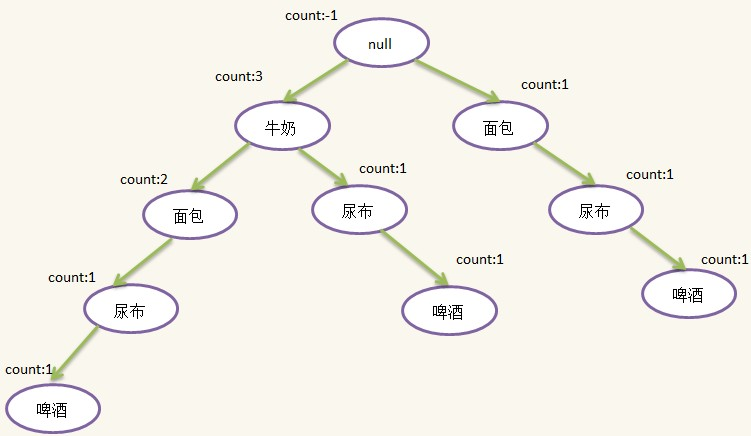
\includegraphics[width = 0.75 \textwidth]{tree4.jpg}
	\caption{第四条记录}
	\label{tree4}
\end{figure}

\item 第五条记录: \{面包,牛奶,尿布,可乐\}

过滤并排序后为: \{牛奶,面包,尿布\}, 检查发现根结点有\{牛奶\}儿子, \{牛奶\}结点有\{面包\}儿子, \{面包\}结点有\{尿布\}儿子, 因此本次插入不需要新建结点只需更新count即可, 示意图如下图\ref{tree5}.
\begin{figure}[!htb]
	\centering
	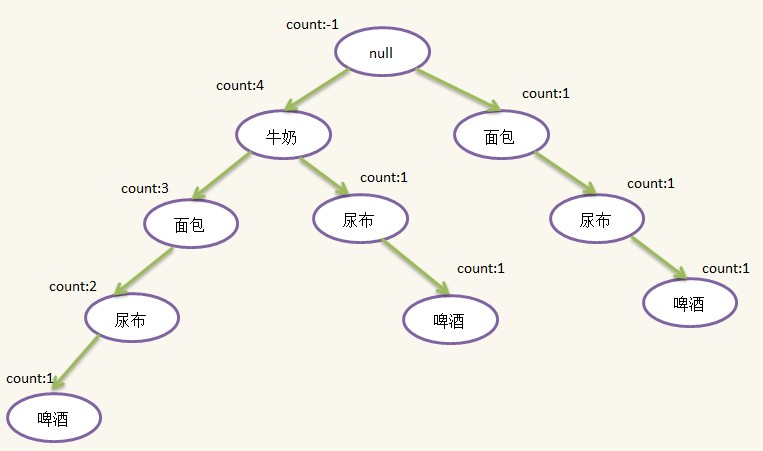
\includegraphics[width = 0.75 \textwidth]{tree5.jpg}
	\caption{第五条记录}
	\label{tree5}
\end{figure}

\end{enumerate}

按照上面的步骤, 我们已经基本构造了一棵FP-Tree, 树中每条路径代表一个项集, 因为许多项集有公共项, 而且出现次数越多的项越可能是公共项, 因此按出现次数由多到少的顺序可以节省空间, 实现压缩存储, 另外我们需要一个表头和对每一个 idName 相同的结点做一个线索, 方便后面使用, 线索的构造也是在建树过程形成的, 但为了简化FP-Tree的生成过程, 上面并没有提到, 但实际编程时要考虑到, 添加线索和表头的FP-Tree如下图\ref{fptree}.
\begin{figure}[!htb]
	\centering
	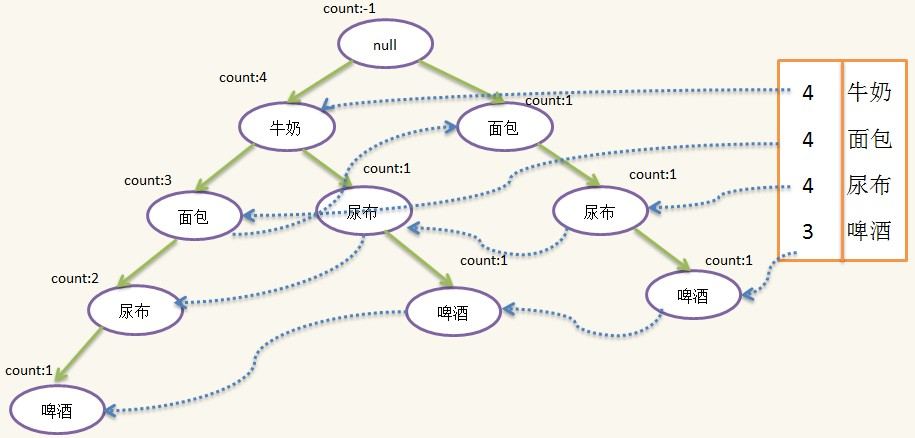
\includegraphics[width = 0.75 \textwidth]{fptree.jpg}
	\caption{FP-Tree}
	\label{fptree}
\end{figure}

至此, 整个FP-Tree就构造好了, 在下面的挖掘过程中我们会看到表头和线索的作用.


\subsubsection{利用FP-Tree挖掘频繁项集}
FP-Tree建好后, 就可以进行频繁项集的挖掘, 挖掘算法称为FP-Growth(Frequent Pattern Growth)算法, 挖掘从表头 header 的最后一个项开始.

\begin{enumerate}[(1)]
\item 此处即从\{啤酒\}开始, 根据\{啤酒\}的线索链找到所有\{啤酒\}结点, 然后找出每个\{啤酒\}结点的分支:\{牛奶, 面包, 尿布, 啤酒: 1\}, \{牛奶, 尿布, 啤酒: 1\}, \{面包, 尿布, 啤酒: 1\}, 其中的“1”表示出现1次, 注意, 虽然\{牛奶\}出现4次, 但\{牛奶, 面包, 尿布, 啤酒\}只同时出现1次, 因此分支的 count 是由后缀结点\{啤酒\}的 count 决定的, 除去\{啤酒\}, 我们得到对应的前缀路径\{牛奶, 面包, 尿布: 1\}, \{牛奶, 尿布: 1\}, \{面包, 尿布: 1\}, 根据前缀路径我们可以生成一颗条件FP-Tree, 构造方式跟之前一样, 此处的数据记录变为
\begin{table}[!htb]
\centering
\label{fp1}
\begin{tabular}{c|c}
	\hline
    % after \: \hline or \cline{col1-col2} \cline{col3-col4} ...
    \textbf{TID} & \textbf{Items}  \\
    \hline
    T1   &  \{牛奶, 面包, 尿布\}  \\
    \hline
    T2   &  \{牛奶, 尿布\} \\
    \hline
    T3   &  \{面包, 尿布\}  \\
	\hline
\end{tabular}
\end{table}

绝对支持度依然是$3$, 同理可得构造得到的 FP-Tree 见图\ref{ar1}.
\begin{figure}[!htb]
	\centering
	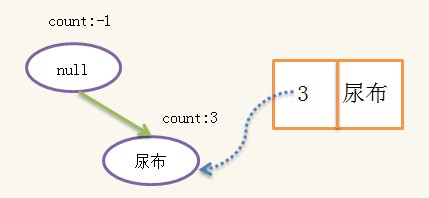
\includegraphics[width = 0.80 \textwidth]{ar1.jpg}
	\caption{啤酒分支}
	\label{ar1}
\end{figure}

构造好条件树后, 对条件树进行递归挖掘, 当条件树只有一条路径时, 路径的所有组合即为条件频繁集, 假设\{啤酒\}的条件频繁集为\{S1,S2,S3\}, 则\{啤酒\}的频繁集为\{S1+\{啤酒\}, S2+\{啤酒\}, S3+\{啤酒\}\}, 即\{啤酒\}的频繁集一定有相同的后缀\{啤酒\}, 此处的条件频繁集为\{\{\}, \{尿布\}\}, 于是\{啤酒\}的频繁集为\{\{啤酒\}, \{尿布, 啤酒\}\}.

\item 接下来找 header 表头的倒数第二个项\{尿布\}的频繁集, 同上可以得到\{尿布\}的前缀路径为: \{面包: 1\}, \{牛奶: 1\}, \{牛奶, 面包: 2\}, 条件FP-Tree的数据集为
\begin{table}[!htb]
\centering
\label{fp2}
\begin{tabular}{c|c}
	\hline
    % after \: \hline or \cline{col1-col2} \cline{col3-col4} ...
    \textbf{TID} & \textbf{Items}  \\
    \hline
    T1   &  \{面包\}  \\
    \hline
    T2   &  \{牛奶\} \\
    \hline
    T3   &  \{牛奶, 面包\}  \\
    \hline
    T3   &  \{牛奶, 面包\}  \\
	\hline
\end{tabular}
\end{table}

注意\{牛奶, 面包: 2\}, 即\{牛奶, 面包\}的 count 为2, 所以在\{牛奶, 面包\}重复了两次, 这样做的目的是可以利用之前构造FP-Tree的算法来构造条件FP-Tree, 不过这样效率会降低, 试想如果\{牛奶, 面包\}的 count 为20000, 那么就需要展开成20000条记录, 然后进行20000次 count 更新, 而事实上只需要对 count 更新一次到20000即可.这是实现上的优化细节, 实践中当注意.构造的条件FP-Tree为图\ref{ar2}.
\begin{figure}[!htb]
	\centering
	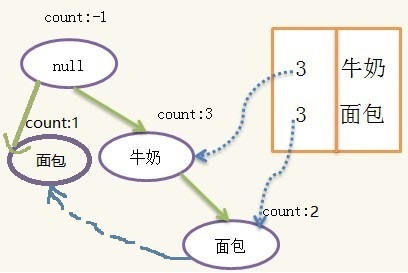
\includegraphics[width = 0.80 \textwidth]{ar2.jpg}
	\caption{尿布分支}
	\label{ar2}
\end{figure}

此图与原作者的不同, 应该是原作者错了, 最后编程输出的结果是对的. 我手动用画图对原图做了修改(捂脸逃).

由此图得到\{尿布\}的频繁项集为\{\{牛奶, 尿布\}, \{面包, 尿布\}\}.

\end{enumerate}

重复以上步骤, 对 header 表头的每个项进行挖掘, 即可得到整个频繁项集, 可以证明, 频繁项集即不重复也不遗漏.

事实上, 以上由FP-Tree挖掘频繁项集的方法来自\url{http://www.cnblogs.com/fengfenggirl/p/associate_fpgowth.html}, FP-Tree 的构建也来自于此, 但是其挖掘频繁项集的方法讲的不是很清楚, 最后一张图也有错误, 所以具体如何由 FP-Tree 挖掘得到频繁项集, 可以参考另一篇文章\url{http://bubuko.com/infodetail-305741.html}.



\section{对关联规则的补充}
以上我们所讨论的关联规则一般称为简单关联, 实际上, 还有两种比较常见的关联规则, 即序列关联(比如时序关联)和因果关联. 下面稍微介绍一下.


\subsection{序列关联规则}
所谓序列关联规则(Frequent Sequential Pattern), 是希望找到序列相关(比如时序)的关联规则, 类似于表\ref{beers}, 序列关联的数据集可能如下表\ref{seqex}所示.
\begin{table}[!htb]
\centering
\caption{序列关联数据集}
\label{seqex}
\begin{tabular}{c|l}
	\hline
    % after \: \hline or \cline{col1-col2} \cline{col3-col4} ...
    \textbf{SID} & \textbf{Sequences}  \\
    \hline
    T1 & $<\{a,b\}, \{c\}, \{f\}, \{g\}, \{e\}>$  \\
    \hline
    T2 & $<\{a,d\}, \{c\}, \{b\}, \{a,b,e,f\}>$  \\
    \hline
    T3 & $<\{a\}, \{b\}, \{f\}, \{e\}>$  \\
    \hline
    T4 & $<\{b\}, \{f,g\}>$  \\ 
	\hline
\end{tabular}
\end{table}


挖掘序列关联规则, 关键的也是挖掘频繁项集, 算法也有很多, 比如 GSP(Generalized Sequential Patterns), SPADE(Sequential PAttern Discovery using Equivalence classes), 其中也会引入支持度和置信度的定义, 与简单关联很类似, 比如表\ref{seqex}的关联规则如表\ref{seqrule}所示.
\begin{table}[!htb]
\centering
\caption{序列关联规则}
\label{seqrule}
\begin{tabular}{clll}
	\hline
    % after \: \hline or \cline{col1-col2} \cline{col3-col4} ...
    \textbf{规则编号} & \textbf{规则} & \textbf{支持度} & \textbf{置信度} \\
    \hline
    R1  & $\{a, b, c\} \rightarrow \{e\}$  & 0.5  &  1.0 \\
    \hline
    R2  & $\{a\} \rightarrow \{c,e,f\}$  & 0.5  & 0.67  \\
    \hline
    R3  & $\{a,b\} \rightarrow \{e,f\}$  & 0.5  & 1.0  \\
    \hline
    R4  & $\{b\} \rightarrow \{e,f\}$  & 0.75  & 0.75 \\ 
    \hline
    R5  & $\{a\} \rightarrow \{e,f\}$  & 0.75  & 1.0 \\ 
    \hline
    R6  & $\{c\} \rightarrow \{f\}$  & 0.5  & 1.0 \\ 
    \hline 
    R7  & $\{a\} \rightarrow \{b\}$  & 0.5  & 0.67 \\ 
    \hline
    \vdots  &  \vdots  &  \vdots  &  \vdots \\
	\hline
\end{tabular}
\end{table}


\subsection{约束关联规则}
当数据集很大的时候, 我们可能会得到很多关联规则, 即使加上了支持度和置信度的约束也是如此, 也就是说得到的关联规则可能并不是我们感兴趣的. 因此, 我们希望加上一些额外的约束, 这便是基于约束的关联规则挖掘. 

我们已经多次提到, 挖掘关联规则的关键是挖掘频繁项集, 因此一般的约束条件也是针对频繁项集而言的. 比如事务交易数据库如下表\ref{constrain}
\begin{table}[!htb]
\centering
\caption{交易数据库}
\label{constrain}
\begin{tabular}{c|l}
	\hline
    % after \: \hline or \cline{col1-col2} \cline{col3-col4} ...
    \textbf{TID} & \textbf{Items}  \\
    \hline
    T1 & $a, b, c$ \\
    \hline
    T2 & $b, c, d, e$ \\
    \hline
    T3 & $a, c$ \\
    \hline
    T4 & $b, d, e$ \\
	\hline
\end{tabular}
\end{table}

其中$a, b, c, d, e$表示$5$个产品, 它们的信息如下表\ref{profit}
\begin{table}[!htb]
\centering
\caption{产品信息表}
\label{profit}
\begin{tabular}{cccc}
	\hline
    % after \: \hline or \cline{col1-col2} \cline{col3-col4} ...
    \textbf{产品} & \textbf{成本} & \textbf{售价} & \textbf{利润} \\
    \hline
    $a$   &  30  &  75  & 45 \\
    \hline
    $b$   &  50  &  60  & 10 \\
    \hline
    $c$   &  50  &  30  & -20 \\
    \hline
    $d$   &  40  &  55  & 15 \\
    \hline
    $e$   &  70  &  40  & -30 \\
	\hline
\end{tabular}
\end{table}

对于任何一个项集$\{I\}$, 我们定义一个约束$C(I)$, 要求项集内的物品总利润必须大于$20$.

设定绝对最小支持度为$\mathrm{minSupport} = 2$, 那么项集$\{a, c\}$和项集$\{d, e\}$都是频繁项集, 但是考虑一下约束条件, 可得
\begin{equation*}
C(\{a, c\}) = 25 > 20, \quad C(\{d, e\}) = -15 < 20
\end{equation*}

因此项集$\{a, c\}$满足约束条件, 而项集$\{d, e\}$不满足, 需要舍弃掉.

如何基于约束高效的挖掘频繁项集, 也有很多算法, 比如 Apriori+ 算法, CAP算法等.





\section{总结}
\subsection{参考资料}
\begin{enumerate}[(1)]
\item 维基百科: \url{https://zh.wikipedia.org/zh/%E5%85%B3%E8%81%94%E5%BC%8F%E8%A7%84%E5%88%99}, 讲的挺好的, 虽然一般英文的更全, 但是有的中文词条确实不错.

\item 博客: \url{http://www.cnblogs.com/fengfenggirl/p/associate_apriori.html}, 啤酒与尿布的典型例子, 此外另一篇将 FP-Tree 的生成讲的比较清楚: \url{http://www.cnblogs.com/fengfenggirl/p/associate_fpgowth.html}, 但是得到 FP-Tree 之后, 如何得到频繁项集说的不是很好, 所以我又参考了下文.

\item 网址: \url{http://bubuko.com/infodetail-305741.html}, 对 FP-Growth 算法讲的比较清楚.

\item 维基: \url{https://en.wikibooks.org/wiki/Data_Mining_Algorithms_In_R/Sequence_Mining/SPADE}, 有用 R 语言的 arulesSequences 包的例子, 当然安装了 R 包以后, 直接看帮助里面的例子也行.

\item 博客: \url{http://data-mining.philippe-fournier-viger.com/introduction-frequent-pattern-mining/}, 对简单关联和序列关联有简单介绍.
\end{enumerate}








\begin{thebibliography}{4}
  \bibitem{1} 李荣华.\emph{偏微分方程数值解法}.高等教育出版社(2010) 
  \bibitem{2} Zhilin Li,Zhonghua Qiao,Tao Tang.\emph{Numerical Solutions of Partial Differential Equations-An Introduction to Finite Difference and Finite Element Methods}.(2011)
  \bibitem{3} 孙志忠.\emph{偏微分方程数值解法}.科学出版社(2011)
  \bibitem{4} 陆金甫 关治.\emph{偏微分方程数值解法}.清华大学出版社(2004)
  
\end{thebibliography}

\newpage

\section*{附录}








\end{document}